\documentclass{article}
\usepackage{graphicx} % Required for inserting images

\title{Homework 7}
\author{Ayman Tawaalai}
\date{March 2024}

\begin{document}

\maketitle

\section{Introduction}
The purpose of the given assignment is to study and implement decision trees, random forest, and gradient boosting. The assignment states that the student must manually implement decision trees, random forest, and gradient boosting using the patient data data set.

\section{Decision Trees, Random Forest, and Gradient Boosting}
Decision tree is a supervised learning classification model that uses binary trees. It works by recursively creating child nodes forming a tree structure to sort out itself into a specific label classification. However, there are n different combinations for how the next node should be. To pick the best one information gain is used on all combinations, and the one with the highest gain is chosen to be the next node. Random forest uses multiple decision trees to make a prediction. It attains labels and data points by splitting it and distributing itself among other trees. From there it will build separate trees. When a new point enters the forest it will go through each tree and voting will take place to classify that point. Gradient boosting is a prediction technique that uses a decision tree. It will then use those predictions to create a regression line. 

\section{Implementation}

The first step in implementation was to create an initialization function housed in the node class. This works similarly to a simple binary tree implementation in data structures. 
\begin{figure}
    \centering
    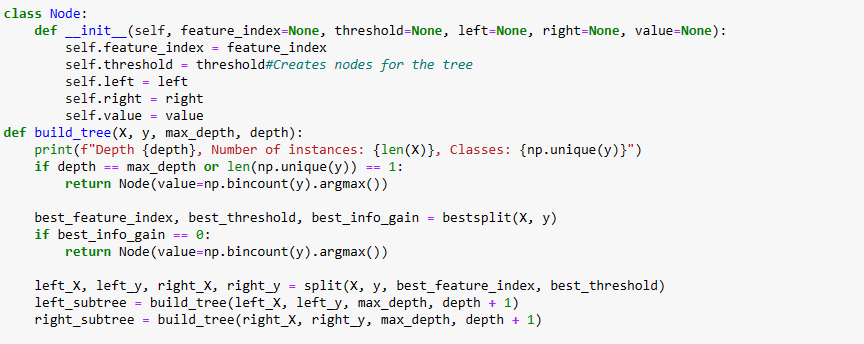
\includegraphics[width=0.5\linewidth]{a.png}
    \caption{Tree Creation}
    \label{fig:enter-label}
\end{figure}
Figure 2 contains the code for implementing decision trees itself. It works by using the build tree function as the main caller. From there it will use the split function to create the multiple combinations. Then when it moved to the best split function it will use the information gain and gini function to calculate which combination is best and select it. That new node will be created using similar binary tree means in the node class.
\begin{figure}
    \centering
    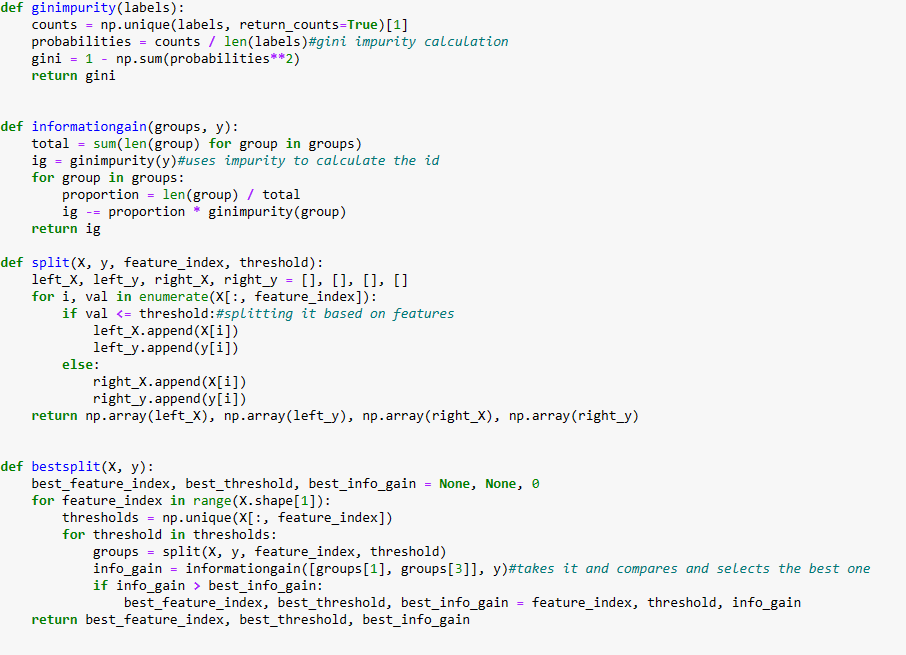
\includegraphics[width=0.5\linewidth]{decision tree.png}
    \caption{Decision Tree}
    \label{fig:enter-label}
\end{figure}
The random forest implementation uses the decision tree code but adds layers onto it for selection. It works by randomly selecting sample indices from the data split and then uses those splits to form multiple decision trees. It will return the forest and the prediction function will conduct majority voting on the forest.
\begin{figure}
    \centering
    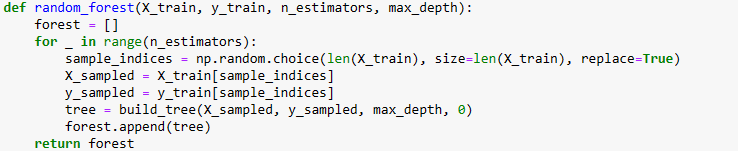
\includegraphics[width=0.5\linewidth]{image.png}
    \caption{Random Forest}
    \label{fig:enter-label}
\end{figure}
\section{Weka}
The data was sent into weka for comparison. The random tree model consistently provided an accuracy of 100\% same with random forest. This is a better accuracy than the one implemented manually in python.
\begin{figure}
    \centering
    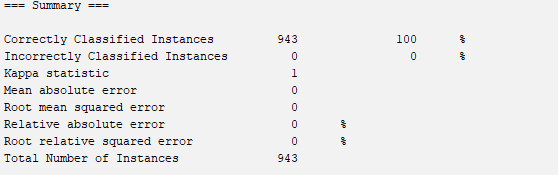
\includegraphics[width=0.5\linewidth]{c.png}
    \caption{Weka Decision Tree}
    \label{fig:enter-label}
\end{figure}
\begin{figure}
    \centering
    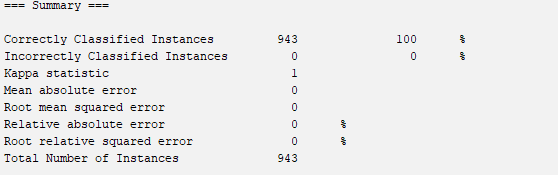
\includegraphics[width=0.5\linewidth]{d.png}
    \caption{Weka Random Forest}
    \label{fig:enter-label}
\end{figure}
\section{Conclusion}
The purpose of the given assignment is to study and implement decision trees, random forest, and gradient boosting. The assignment states that the student must manually implement decision trees, random forest, and gradient boosting using the patient data data set. The manual implementation done did not prove as accurate as Weka, but it is useul. More tuning can be done to improve the accuracy as well.
\end{document}
